\chapter{Hardvertervezés}

\section{Áramköri tervezés}
A prototípus áramkörét próbáltam minél egyszerűbben megvalósítani. Alapvetően két részből áll, a Raspberry PI központú vezérlőáramkörből, ami felelős a szenzorokért és a Raspberry PI-ért, illetve egy nagyobb teljesítményű áramkör egy külön tápról, ami a gearbox működtetéséért felelős.


\begin{figure}[h!]
	\centering
	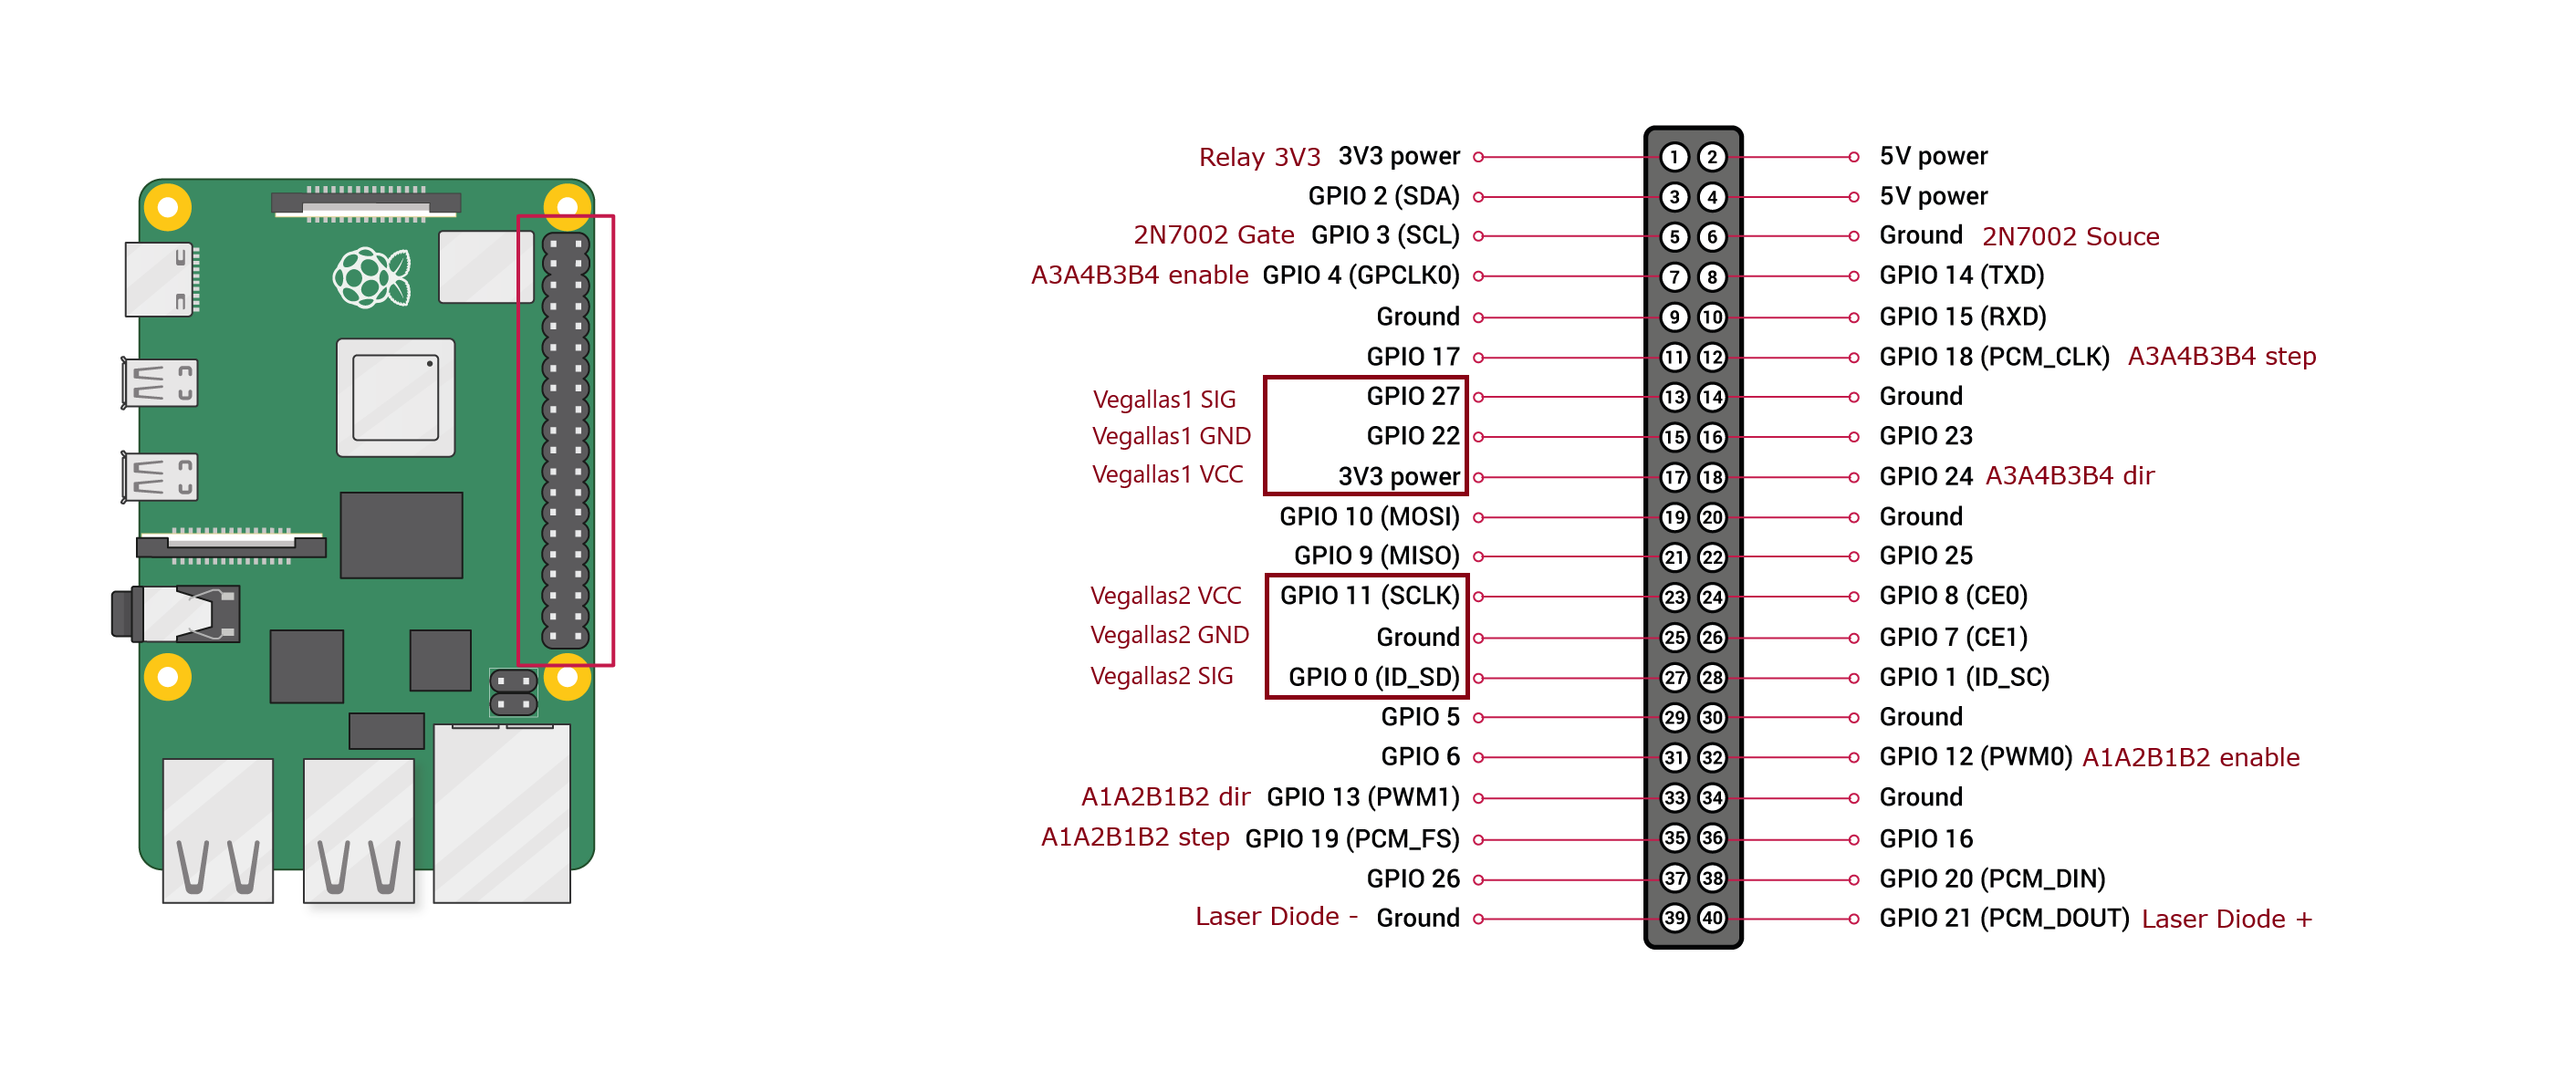
\includegraphics[width=1\linewidth]{elek_pinout}
	\caption{A Raspberry PI lábkiosztása \cite{raspberry4}}
	\label{fig:elek_pinout}
\end{figure}


A prototípus áramköre a \ref{fig:schematic} ábrán látható. A kereskedelemben kapható \textsl{Stepper Motor HAT} nagyban leegyszerűsítette a tervezés folyamatát, a segítségével nem kellett megterveznem a motorvezérlők áramkörét, illetve ezeknek az áramellátását. A \ref{fig:elek_pinout}.ábrán látható, motorokra vonatkozó jelölések szerinti GPIO lábakat a \textsl{Stepper Motor HAT} ugyan lefoglalja, de a kártya tetején lévő tüskesor ugyanúgy elérhető marad, így oda kell figyelnem, hogy ezeket a lábakat ne használjam. \\

\begin{figure}[h!]
	\centering
	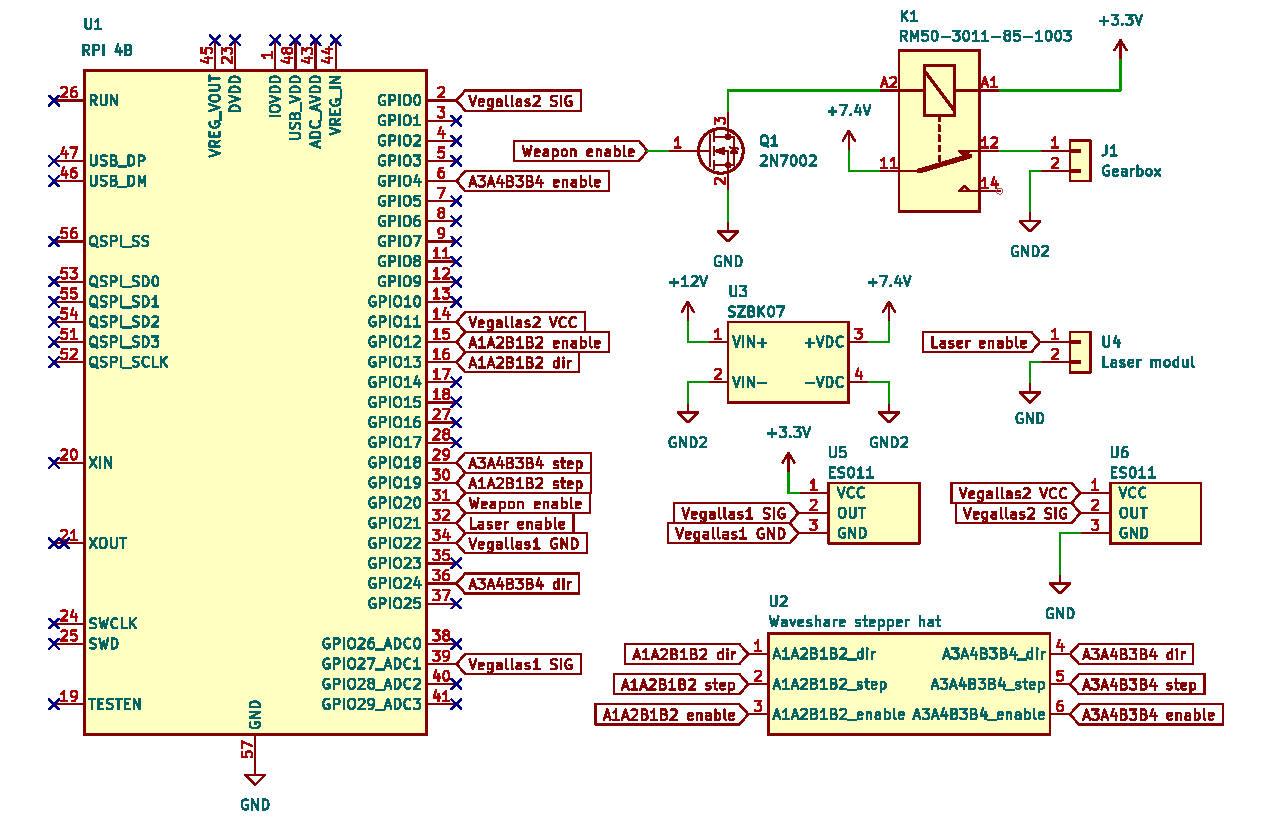
\includegraphics[width=1\linewidth]{schematic2}
	\caption{A prototípus sémarajza}
	\label{fig:schematic}
\end{figure}

Ahogy az ábrán látható, a végálláskapcsolók is a GPIO tüskesorra lettek csatlakoztatva. Az egyiknél a földet helyettesíti GPIO22 láb, a másiknál a 3.3 V-t helyettesíti a GPIO11. Azért kellett ezt a megoldást alkalmaznom, mert a kábel csatlakozója egyben van, nem különálló jumper tüskék.\\

A lézer közvetlenül a GPIO21 lábról működik. Eleinte aggódtam, hogy nem tud elegendő áramot szolgáltatni a dióda működtetéséhez, de szerencsére mégis. Ellenkező esetben ki kellett volna egészítenem az áramkört egy tranzisztorral. \\

A relé kapcsolásához viszont nem volt elegendő a GPIO láb által szolgáltatott áram, így azt egy tranzisztorral vezérlem. Amennyiben logikai magas jelet kap, a relé zárja a gearbox áramkörét, és az elkezd lőni.

Az eszköz sémarajza az alábbi ábrán látható:


\pagebreak

\section{Elektronikai alkatrészek}
\subsubsection*{Mikrovezérlő}
A mikrokontroller kiválasztásánál több opciót vizsgáltam, többek között az {Arduino}, az \textsl{STM-32} és a \textsl{Raspberry PI} modelleket. A követelmények a következőek voltak:

\begin{list}{$\bullet$}{}
	\item Legyen könnyen beszerezhető, mind anyagilag, mind elérhetőség szerint
	\item Megfelelő teljesítmény gépi látás algoritmusokhoz
	\item Elegendő számú GPIO kimenet
	\item Python programozási nyelve támogatása
	\item Ethernet port
\end{list}

Ahogy összehasonlítottam a különböző opciókat, körvonalazódott, hogy a \textsl{Raspberry PI} \cite{raspberry4} lesz a megfelelő megoldás. Az eszköz az \ref{fig:elek_raspberry4b}. ábrán látható. Először is egy gyakorlati szempont szerint, mégpedig hogy egy Raspberry PI 4B modell eredetileg is volt a tulajdonomban 4GB rammal. A gyártó hivatalos fórumán több felhasználó szerint ez már elegendő összetettebb gépi látás algoritmusok futtatására is. \cite{4gbforum} \\

\begin{figure}[h!]
	\centering
	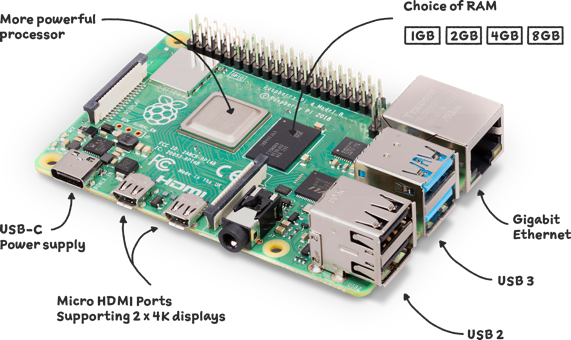
\includegraphics[width=0.5\linewidth]{elek_raspberry4b}
	\caption{Raspberry 4 model B \cite{raspberry4}}
	\label{fig:elek_raspberry4b}
\end{figure}

A kamera illesztése szintén különösen fontos a végtermék működése szempontjából, és ezen a területen magasan kiemelkedik a Raspberry a többi mikrovezérlő közül, mivel a gyártó magán a termékcsaládon belül ajánl több jó minőségű, könnyen beszerezhető kamera modult, amik illesztése már kiforrott az összes Raspberry-hez.\\

Ezentúl a \textsl{Raspberry PI} erősebb, mint a fentebb említett mikrokontrollerek. Linux rendszert futtat, és lehet rajta Python nyelven programozni, ami gépi látás, automatizálás projekteknél hatalmas előny. Számos ki-és bemenete van, ráadásul támogatja a \textsl{Bluetooth}, \textsl{Wi-Fi}, és gigabites \textsl{Ethernet} kapcsolatokat is, nem beszélve a rengeteg bővítő "kabátról", amiket lehet kapni hozzá. Ezek a termék továbbfejlesztését nagyban könnyítik, ráadásul kevesebb munkát kell a nyomtatott áramkör tervezésébe tenni.\\

\subsubsection*{Stepper Motor HAT \cite{stepperhat}}
A NEMA-17 léptetőmotorok vezérlésére több megoldás is létezik, elterjedtek a \textsl{A4988}, \textsl{TMC5160T} és \textsl{DRV8825} típusú vezérlők. Ezeket azonban vagy külön modulként lehet megvásárolni, vagy pedig SMD alkatrészként, ami mellé mindenképpen kell tervezni kiegészítő áramkört. \\

\begin{figure}[h!]
	\centering
	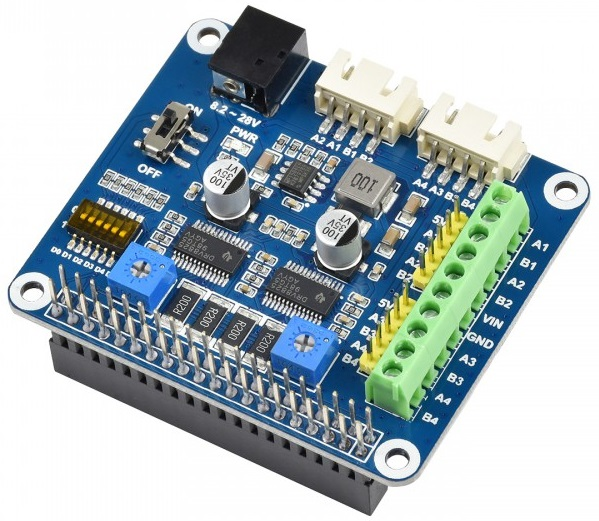
\includegraphics[width=0.4\linewidth]{elek_stepperhat}
	\caption{Waveshare Stepper HAT \cite{stepperhat}}
	\label{fig:elek_stepperhat}
\end{figure}

Azonban a \textsl{Waveshare} cég gyárt egy Raspberry Pi-kompatibilis modult, ami számomra rengeteg segítséget nyújtott. Ez egy külön áramkör, amit a Raspberry GPIO tüskesorára lehet illeszteni. Képes két \textsl{DRV8825} vezérlővel egyszerre kettő léptetőmotort vezérelni. A kártyán lévő kapcsolókkal könnyen lehet állítani külön motoronként a microsteppelést is, amennyiben szükség van rá egészen 1/32-ig. Szoftveresen is lehet állítani a microsteppelést, azonban ehhez forrasztani kellene a kártyára plusz ellenállásokat. A potméterekkel motoronként tudjuk állítani a maximális felvehető áramot, maximum 2.5 A-ig. A kártyán helyet kapott egy standard 5.5 mm-es csatlakozó is, amivel 8.2 V és 28 V közötti feszültséggel lehet táplálni az áramkört. Egy belső regulator chip segítségével a Raspberry PI-t is el lehet látni árammal, így egy tápegységgel tudom működtetni a teljes áramkört. A modulon több lehetőség is van csatlakoztatni a motorokat, akár sorkapoccsal, akár a léptetőmotorok szabvány csatlakozójával. Ezentúl lehetővé teszi a Raspberry PI GPIO lábainak elérését, csupán arra kell odafigyelni, melyikeket használja. Az eszközről a \ref{fig:elek_stepperhat}. ábrán látható illusztráció. Az eszköz el lett látva különböző biztonsági funkciókkal, pl. túláram védelemmel, magas hőmérséklet elleni védelemmel, illetve alulfeszültség lockout-tal. \\

A gyártó szintén elérhetővé tett illesztőszoftvereket több eszközre, több motortípusra, amit a későbbiekben én is tudtam használni.

\subsubsection*{Táp}

A prototípust két tápegységről működtetem. Az egyik a Raspberry PI, a léptetőmotorok és a szenzorok áramellátásáért, ez egy standard 5.5 mm-es csatlakozóval ellátott laptop töltő. 14.5 V tápfeszültséget és maximum 5 A áramot képes biztosítani, amely bőven elegendő a vezérlőelektronika ellátására. A másik táp egy \textsl{HP ps-3701-1} 12 V-os redundáns szervertáp 725 W teljesítménnyel. 

\subsubsection*{DCDC konverter}
A gearbox gyárilag 7.4 V-ról tud működni, tehát a kapott 12V-ot át kellett alakítani. Erre egy \textbf{SPX-20A} típusú DC-DC step-down konverted modult alkalmaztam. Ennek a maximum kimeneti árama 20A, maximum teljesítménye 300W. Elméletileg a gearbox felvett árama tüskeszerűen fellőhet 15A fölé, ami fölött már ventilátoros hűtés javasolt, de mivel ez nem lenne tartós, így én úgy döntöttem, ezt kihagyom. A kimeneti feszültséget és az áramkorlátot lehet állítani a kártyán található potméterekkel, de gyakorlatban csak a feszültséget állítottam. Minél nagyobb feszültséggel hajtom a gearboxot, annál gyorsabban pörög a motor, tehát annál nagyobb gyakorisággal lövi ki a golyókat. A gearbox és a táp kábeleit a kártyán található csavaros terminállal csatlakoztattam, maga a modul pedig a kereten kapott helyet, a Raspberry PI konzolján.

\subsubsection*{Kamera}
A rendszer által használt kamera egy \textsl{Raspberry Pi Camera Module 2} volt.\cite{raspberrycam} Ez a modul 8 MP-es \textsl{Sony IMX219} szenzorral rendelkezik, amivel 3266 x 2450 felbontású állóképet tud készíteni. Képes Full HD videót felvenni 30 fps-el, HD-t 60 fps-el, vagy 640x480 felbontást 90 fps-el. A modul a \ref{fig:elek_raspberrycam}. ábrán látható.

\begin{figure}[h!]
	\centering
	
\includegraphics[width=1\linewidth]{elek_raspberrycam}
	\caption{Raspberry Pi Camera Module 2 \cite{raspberrycam}}
	\label{fig:elek_raspberrycam}
\end{figure}

A kamera befoglaló mérete szerelési furatai és CSI portja megegyezik a többi Raspberry kamerával, így a továbbfejlesztés esetén könnyedén lehet őket cserélni.

\subsubsection*{Végálláskapcsoló}
A prototípus bekapcsolásánál fontos, hogy beálljon egy kezdőpozícióba, és ahhoz képest tudjuk viszonyítani a mozgását. Ezt én a két tengelyen 1-1 végálláskapcsolóval oldottam meg. Ezek a modulok könnyen szerelhetőek a 3D nyomtatott vázra, és az alapján adnak jelet, valami van-e az optokapu között. A Raspberry GPIO lábaira könnyedén lehet őket bekötni jumper kábelek segítségével.

